\documentclass{article}
\usepackage[a4paper, top=2cm, bottom=3cm]{geometry}

\usepackage[ngerman]{babel}
\usepackage{csquotes}

\usepackage{booktabs}

\usepackage{amssymb}
\usepackage{amsmath}
\usepackage{mathtools}
\usepackage{enumitem}

\usepackage{hyperref}

\usepackage{graphicx}
\usepackage{wrapfig}

\usepackage{parskip}
\usepackage{fancyhdr}
\usepackage{vmargin}

\usepackage{pgfplots}
\pgfplotsset{compat=1.18}

\usepackage{siunitx}
\sisetup{locale = DE}

\usepackage{biblatex}
\DefineBibliographyStrings{ngerman}{
  urlseen = {Abruf vom}
}
\addbibresource{quellen.bib}

\newcommand{\proofeq}{\overset{!}{=}}
\newcommand{\proofeqv}{\overset{!}{\Leftrightarrow}}
\newcommand{\equivalent}{\overset{\scriptscriptstyle\wedge}{=}}
\DeclarePairedDelimiter\ceil{\lceil}{\rceil}
\DeclarePairedDelimiter\floor{\lfloor}{\rfloor}

\date{25.03.2022}
% Physikalisches Grundpraktikum I \\ (Mechanik und Thermodynamik)
\title{Versuch 1: Mechanische Schwingungen}
\author{Wafaa Al Nachwati (8102531) \\ Finn Bietz (8104485) \\ Finn Wagner (8102237)}

\begin{document}

    \makeatletter
\let\thetitle \@title{}
\let\theauthor \@author{}
\let\thedate \@date{}
\makeatother

\fancyhf{}

    \begin{titlepage}
        \centering
        \vspace*{0.5 cm}
        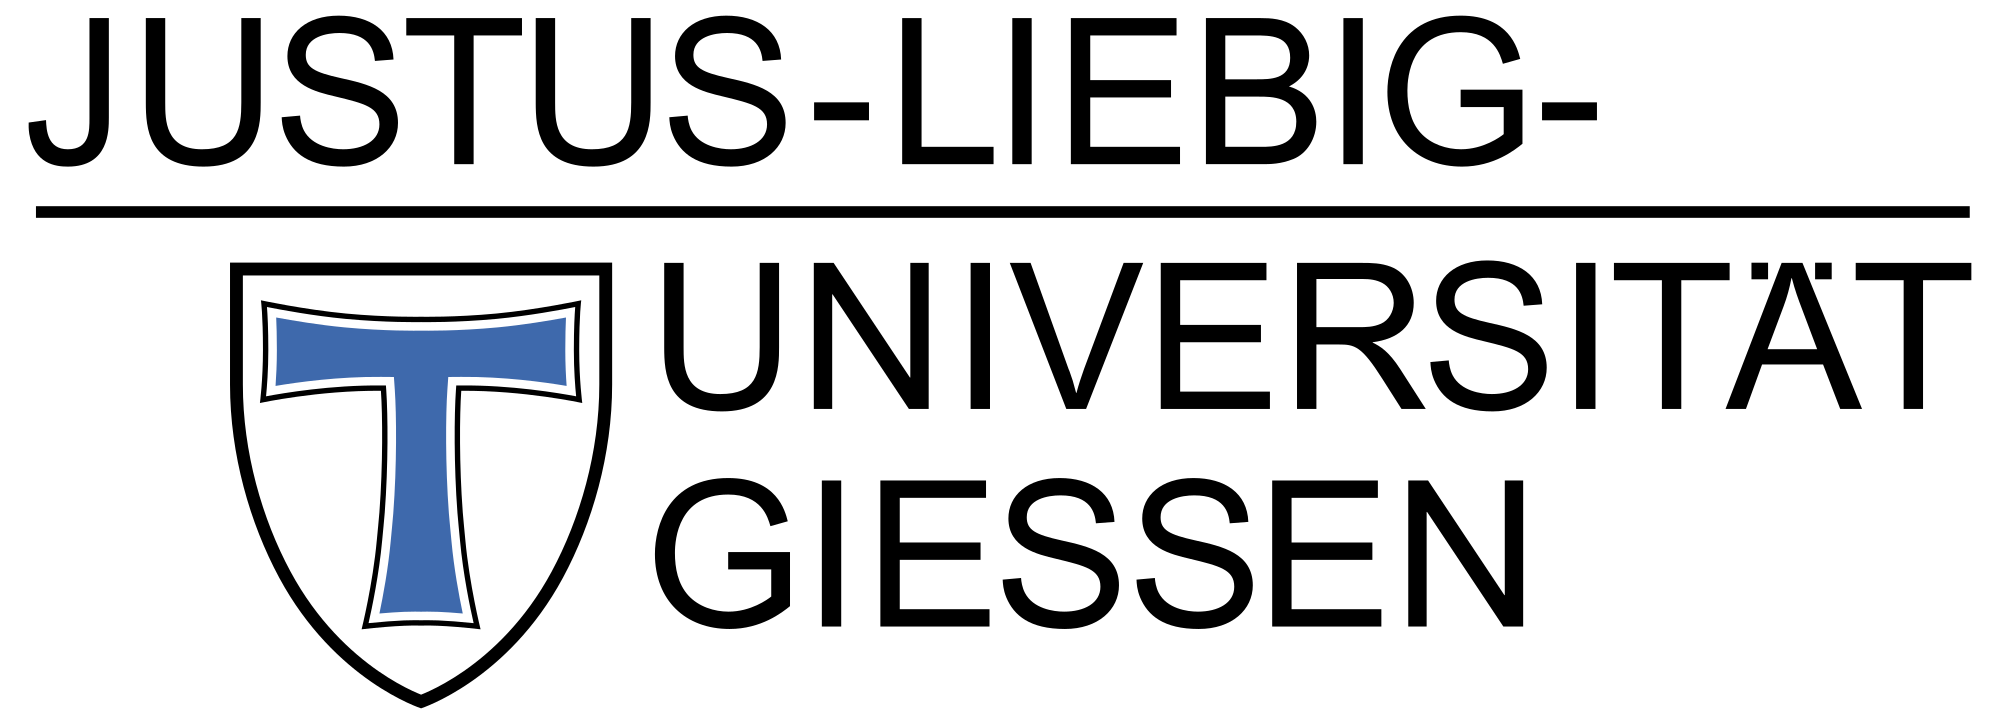
\includegraphics[ width = 0.6 \textwidth ]{fotos/uni-logo.png} \\ [2.0 cm]

        Protokoll zu: \\
        \begin{center}    
            \textsc{ \Large Physikalisches Grundpraktikum I \\ (Mechanik und Thermodynamik)} \\ [2.0 cm]
        \end{center}
        
        \rule{\linewidth}{0.2 mm} \\ [0.4 cm]
        { \huge \bfseries \thetitle} \\
        \rule{\linewidth}{0.2 mm} \\ [1.5 cm]
                
        \begin{minipage}{ 0.4 \textwidth }
            \begin{flushright} \large
                \emph{Protokoll von: } \\
                \theauthor{}
            \end{flushright}
        \end{minipage} \\ [2 cm]
        
    \end{titlepage}

	\maketitle

    \section{Versuchsziel und Versuchsmethode}
        In dieser Versuchsreihe mit drei Versuchen beschäftigen wir uns mit Federn und dem Hookeschen Gesetz und Federkonstanten,
        sowie harmonischen Oszillatoren und Schwebungen. \\
        Im ersten Versuch bestimmen wir eine Federkonstante durch mehrere Messungen wie weit die Feder bei einer durch eine Masse
        erzeugten Kraft ausgelenkt wird.
        Im zweiten Versuch betrachten wir einen harmonischen Oszillator. Er besteht aus einem zwischen zwei Federn eingespannten Gleiter.
        Aus der Schwingungsdauer des Gleiters berechnen wir seine Masse.
        Da der Gleiter gedämpft ist messen wir auch die Zeit die es braucht bis die Amplitude der Schwingung auf die Hälfte zurückgegangen ist.
        Aus dieser Zeit berechnen wir die Dämpfungskonstante \(b\). \\
        Für den letzten Versuch fügen wir noch einen weiteren über eine Feder mit geringer Federkonstante verbundenen Gleiter hinzu.
        Wir vermessen die beiden Eigenmoden des Systems und und vergleichen sie mit dem theoretischen Wert. 
        Neben den Eigenmoden messen wir auch noch die Schwebungsfrequenz des Systems und vergleichen auch diese mit unseren theoretischen Vorhersagen.

    \section{Allgemeiner Aufbau}
        Die Experimente in diesem Versuch, werden um Reibungseffekte zu minimieren und das messen zu erleichtern auf einer Luftkissenbahn durchgeführt.
        % TODO: FOTO
        Zur genaueren Auswertung verwenden wir eine digitale Messapparatur. Sie misst mit einer CCD-Kamera über eine reflektierende Folie am Gleite deren Position.

    \section{Federkonstante}
        \subsection{Durchführung}
        \subsection{Messergebnisse}
        \subsection{Auswertung}
            \subsubsection{Graphische Auswertung}
            \subsubsection{Fehlerrechnung} 
            \subsubsection{Endergebnis}
            Federkonstante

    \section{Harmonische Oszillation}
        \subsection{Durchführung}
        \subsection{Messergebnisse}
        \subsection{Auswertung}
            \subsubsection{Fehlerrechnung} 
            \subsubsection{Endergebnis}
                Masse des Gleiters \\
                Dämpfungskonstante \(b\)

    \section{Gekoppelter Harmonische Oszillator}
        \subsection{Durchführung}
        \subsection{Messergebnisse}
        \subsection{Auswertung}
            \subsubsection{Fehlerrechnung}
            ?????????????????????
            \subsubsection{Endergebnis}
                Ergebnisse vergleichen

\end{document}